\section{kNN Models}
By nonparametric models we generally refer to \textbf{Nearest Neighbor Models}, this type of approach is called "lazy learning" in that it does not build any model, all the work is done during the prediction phase.

\subsection{Nierest Neighbors}
A simple implementation of a Nearest Neighbor algorithm simply corresponds to calculating the minimum distance between the input and the examples in the dataset and assigning the class of the nearest example to the input.
This method does not go to explicitly create decision boundaries but they can be calculated and shown using a Voronoi diagram.
\begin{center}
    \begin{tabular}{c}
        \\ 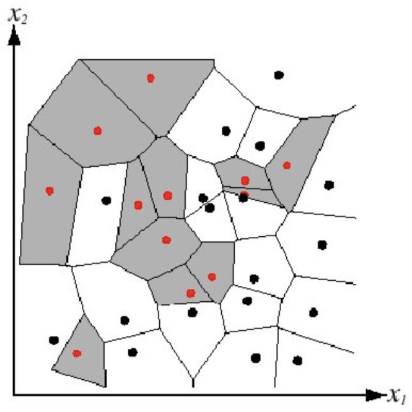
\includegraphics[width=0.4\textwidth]{images/kNN1.png} \\ \\
    \end{tabular}
\end{center}

\subsection{k-Nearest Neighbors}
The $k$ closest examples are considered to classify the input.
The input is ranked according to the class of the majority of the $k$ closest examples.
However, too large a $k$ can be a problem since there is a risk that considering too many examples always wins the most frequent class in the dataset.
A good rule for choosing the $k$ is as follows:
\begin{equation} \tag*{}
    k = \sqrt{m}
\end{equation}
where $m$ is the number of examples in the dataset.
\begin{center}
    \begin{tabular}{c c c}
        \\
        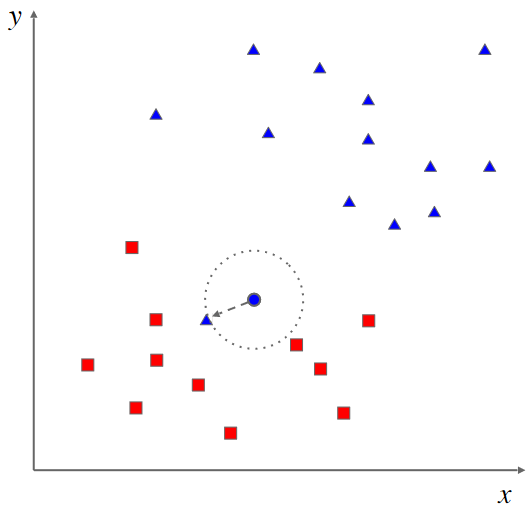
\includegraphics[width=0.3\textwidth]{images/kNN2.png} &
        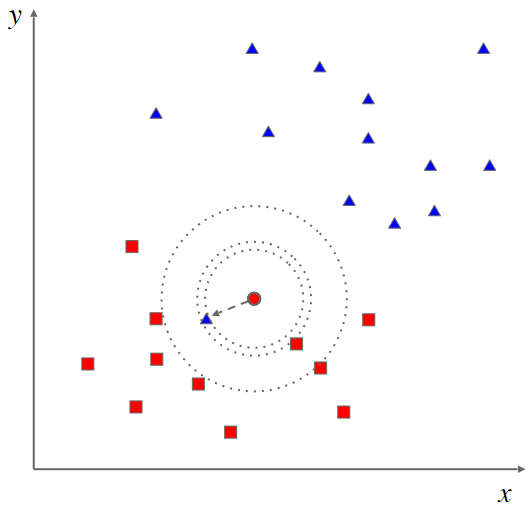
\includegraphics[width=0.3\textwidth]{images/kNN3.png} &
        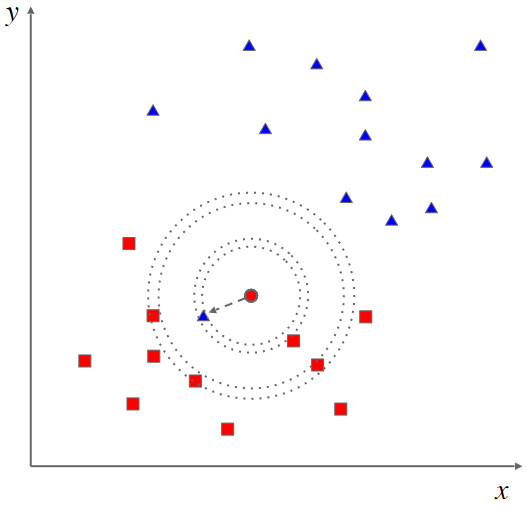
\includegraphics[width=0.3\textwidth]{images/kNN4.png}
    \end{tabular} 
\end{center}

\newpage
\subsection{Python Implementation}
\begin{lstlisting}[language=Python]
import numpy as np

class NearestNeighbor:

    def __init__(self):
        pass

    def train(self, X, y):
        self.Xtr = X
        self.ytr = y

    def predict(self, X):
        num_test = X.shape[0]
        Ypred = np.zeros(num_test, dtype = self.ytr.dtype)
        for i in range(num_test):
            distances = np.sum(np.abs(self.Xtr - X[i,:]), axis = 1)
            min_index = np.argmin(distances)
            Ypred[i] = self.ytr[min_index]
        return Ypred
\end{lstlisting}

\subsection{Pros and Cons}
\begin{multicols}{2}
    \begin{itemize}
        \item Creates complex decision boundaries and adapts to data density
        \item With many samples it works well
        \item[] 
        \item[] 
    \end{itemize} 
    \columnbreak
    \begin{itemize}
        \item Sensitive to noise between classes and different feature scales
        \item In high dimensionality datasets is less effective
        \item Complexity scales linearly with the number of training data, very expensive at test time
        \item Inductive bias (assumes neighboring samples in feature space have the same class)
    \end{itemize}
\end{multicols}

\newpage